\documentclass{article}
\usepackage{amsmath}
\usepackage{graphicx}
\usepackage{siunitx} % Required for alignment
\usepackage{multirow}
\usepackage{booktabs} % pretty tables

\sisetup{
  round-mode = places, % Rounds numbers
  round-precision = 2, % up to two places
}

\title{The Everything Template}
\date{2017-12-15}
\author{Felix Zhou}

\begin{document}
\pagenumbering{gobble}
\maketitle
\newpage
\tableofcontents
\newpage
\pagenumbering{arabic}

\section{Figures}

\begin{figure}[h!]
 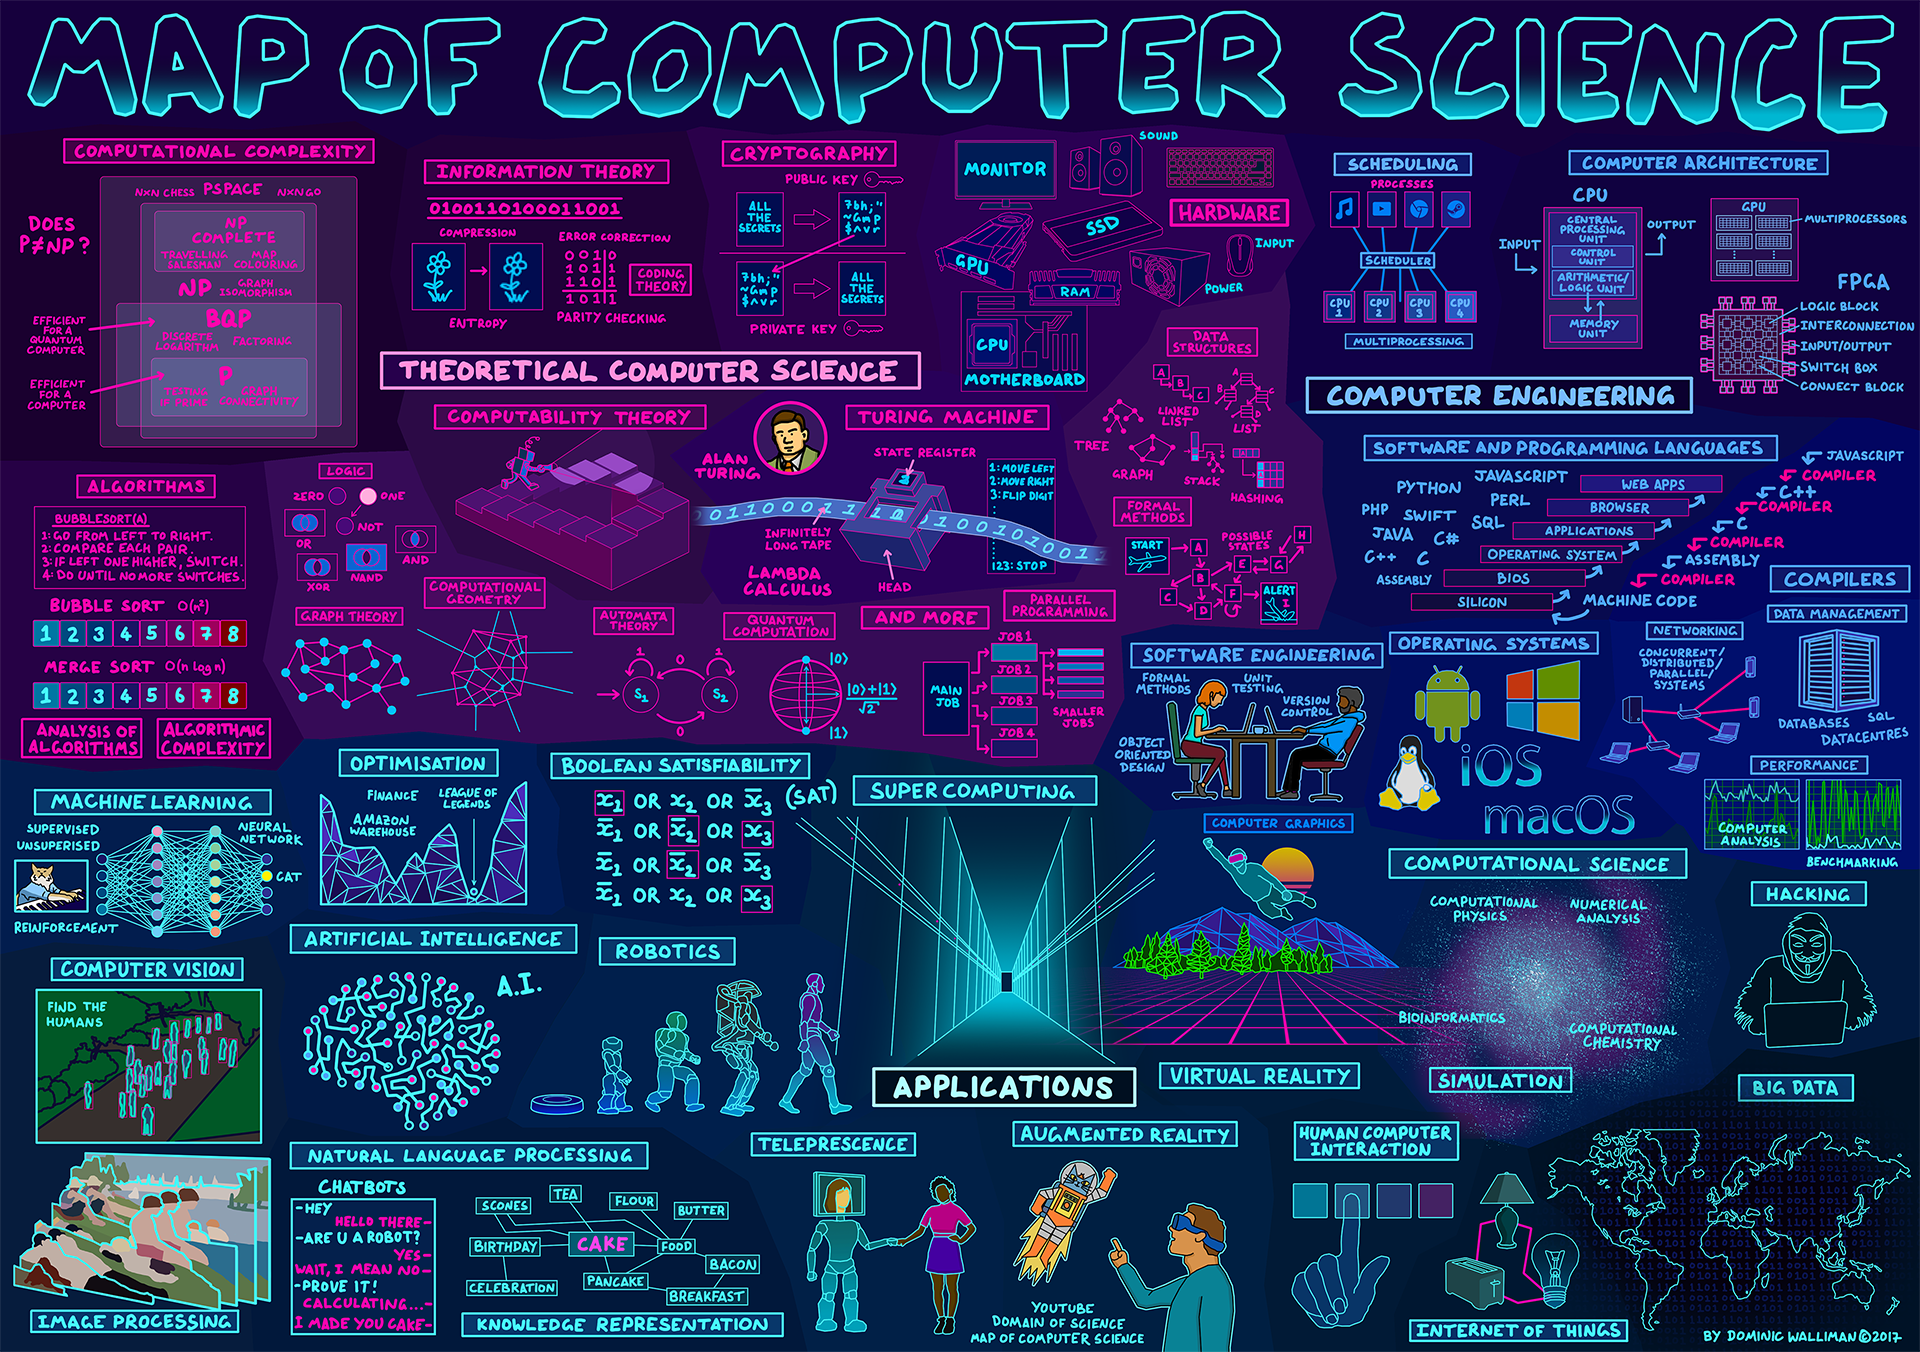
\includegraphics[width=\linewidth]{Map.png}
 \caption{A Map.}
 \label{fig:Map of CS}
\end{figure}

\section{Text and Inline Math}

Hello World!
$f(x) = x^2$ fam!!
I absolutely hate my life:)

\subsection{Common Mathematical Features}

\begin{align*}
 f(x) & = x^2                    \\
 g(x) & = \frac{1}{x}            \\
 F(x) & = \int^a_b \frac{x^3}{3}
\end{align*}

\section{Paragraphs}

\paragraph{paragraph 1}

\begin{equation*}
 f(x) = 6x^2
\end{equation*}

Yay! a paragraph!!

\subparagraph{subparagraph}

$\left(\frac{1}{\sqrt{x}}\right)$\\
$\left(\left(\lambda\left(x\right)xx\right)\left(\lambda\left(x\right)xx\right)\right)$
Is there any end? That is the question!!

\section{Matrices}

$\left[
  \begin{matrix}
   1 & 0 \\
   0 & 1
  \end{matrix}
  \right]$

\section{Footnotes}

This is some example text...\footnote{\label{myfootnote}...and its corresponding footnotes}

\section{Tables}

\begin{table}[h!]
 \begin{center}
  \caption{Multi-row/column table using booktabs}
  \label{tab:table1}
  \begin{tabular}{l|S|r} % <-- Alignments: 1st column left, 2nd middle and 3rd right, with vertical lines in between
   \textbf{Value 1}                           & \textbf{Value 2} & \textbf{Value 3} \\
   $\alpha$                                   & $\beta$          & $\epsilon$       \\
   \toprule
   \multirow{2}{*}{69}                        & 100.567          & z                \\
                                              & 1110.1           & a                \\
   \midrule
   \multicolumn{2}{c|}{12}                    & a.1                                 \\
   \midrule
   \multicolumn{2}{c|}{\multirow{2}{*}{1234}} & a                                   \\ % <-- Multicolumn spanning 2 columns, content multirow spanning two rows
   \multicolumn{2}{c|}{}                      & b                                   \\ % <-- Multicolumn spanning 2 columns with empty content as placeholder
   \bottomrule
   2                                          & 10.1             & b                \\
   3                                          & 23.113231        & c                \\
   4                                          & \pi              & d                \\
  \end{tabular}
 \end{center}
\end{table}



\newpage
\begin{appendix}
 \listoffigures
 \listoftables
\end{appendix}

\end{document}
